% -*- coding: UTF-8 -*-
% hurlex-chapt11.tex
% hurlex 开发文档 第11章内容

\section {内核堆管理的实现}

\par 前几章实现了内存的简单管理,但是目前的内存分配是按页为单位的,这样在需要分配小内存的时候比较容易造成内部碎片。这章我们来实现内核的堆管理算法,目的是为了小内存的分配。除了简单的分配内存之外,还需要考虑在内存释放的时候,对连续的内存进行合并。并且堆要实现在空闲内存过多的时候把物理页释放给物理内存管理模块。

\par 关于堆的实现有很多种,我们选择最简单的侵入式链表管理方法。如果你觉得可以胜任更好的算法完全可以自由发挥,而且之前的物理内存管理算法完全可以实现为伙伴系统。不过为了照顾大多数读者,我们选择简单的方式实现。当然,通过简单的算法熟悉了物理机制之后,完全可以抛开这些简单实现,去实现更好的算法。

\par 首先,在每一个申请的内存块之前插入一个描述当前内存块的结构体。结构体定义以及相关的函数声明如下:

\begin{lstlisting}[language = C, caption = include/heap.h]
#ifndef INCLUDE_HEAP_H_
#define INCLUDE_HEAP_H_

#include "types.h"

// 堆起始地址
#define HEAP_START 0xE0000000

// 内存块管理结构
typedef
struct header {
	struct header *prev; 	// 前后内存块管理结构指针
	struct header *next;
	uint32_t allocated : 1;	// 该内存块是否已经被申请
	uint32_t length : 31; 	// 当前内存块的长度
} header_t;

// 初始化堆
void init_heap();

// 内存申请
void *kmalloc(uint32_t len);

// 内存释放
void kfree(void *p);

// 测试内核堆申请释放
void test_heap();

#endif 	// INCLUDE_HEAP_H_
\end{lstlisting}

\par 结构体的定义里使用了C语言的位域定义,因为表示这块内存有没有被使用只需要1个bit就可以,这样节省内存。这里定义的堆的函数形式很简单,就不详细解释了。需要注意的是这里定义了虚拟堆起始地址为0xE0000000,它是内核页表没有使用的空闲区域。

\par 接下来是具体实现。除了以上的外部接口函数,还需要在实现文件里声明以下内部函数:

\begin{lstlisting}[language = C, caption = mm/heap.c]
#include "debug.h"
#include "pmm.h"
#include "vmm.h"
#include "heap.h"

// 申请内存块
static void alloc_chunk(uint32_t start, uint32_t len);

// 释放内存块
static void free_chunk(header_t *chunk);

// 切分内存块
static void split_chunk(header_t *chunk, uint32_t len);

// 合并内存块
static void glue_chunk(header_t *chunk);

static uint32_t heap_max = HEAP_START;

// 内存块管理头指针
static header_t *heap_first;
\end{lstlisting}

\par 这些内部函数只在堆的内部被调用,所以被声明为static,我们之前也强调过,不需要向外部暴露的函数最好用static限制其作用域。我们直接贴出相关函数的实现:

\begin{lstlisting}[language = C, caption = mm/heap.c]
... ...

void init_heap()
{
	heap_first = 0;
}

void *kmalloc(uint32_t len)
{
	// 所有申请的内存长度加上管理头的长度
	// 因为在内存申请和释放的时候要通过该结构去管理
	len += sizeof(header_t);

	header_t *cur_header = heap_first;
	header_t *prev_header = 0;

	while (cur_header) {
		// 如果当前内存块没有被申请过而且长度大于待申请的块
		if (cur_header->allocated == 0 && cur_header->length >= len) {
			// 按照当前长度切割内存
			split_chunk(cur_header, len);
			cur_header->allocated = 1;
			// 返回的时候必须将指针挪到管理结构之后
			return (void *)((uint32_t)cur_header + sizeof(header_t));
		}
		// 逐次推移指针
		prev_header = cur_header;
		cur_header = cur_header->next;
	}

	uint32_t chunk_start;

	// 第一次执行该函数则初始化内存块起始位置
	// 之后根据当前指针加上申请的长度即可
	if (prev_header) {
		chunk_start = (uint32_t)prev_header + prev_header->length;
	} else {
		chunk_start = HEAP_START;
		heap_first = (header_t *)chunk_start;
	}

	// 检查是否需要申请内存页
	alloc_chunk(chunk_start, len);
	cur_header = (header_t *)chunk_start;
	cur_header->prev = prev_header;
	cur_header->next = 0;
	cur_header->allocated = 1;
	cur_header->length = len;
	
	if (prev_header) {
		prev_header->next = cur_header;
	}

	return (void*)(chunk_start + sizeof(header_t));
}

void kfree(void *p)
{
	// 指针回退到管理结构,并将已使用标记置 0
	header_t *header = (header_t*)((uint32_t)p - sizeof(header_t));
	header->allocated = 0;

	// 粘合内存块
	glue_chunk(header);
}

void alloc_chunk(uint32_t start, uint32_t len)
{
	// 如果当前堆的位置已经到达界限则申请内存页
	// 必须循环申请内存页直到有到足够的可用内存
	while (start + len > heap_max) {
		uint32_t page = pmm_alloc_page();
		map(pgd_kern, heap_max, page, PAGE_PRESENT | PAGE_WRITE);
		heap_max += PAGE_SIZE;
	}
}

void free_chunk(header_t *chunk)
{
	if (chunk->prev == 0) {
		heap_first = 0;
	} else {
		chunk->prev->next = 0;
	}

	// 空闲的内存超过 1 页的话就释放掉
	while ((heap_max - PAGE_SIZE) >= (uint32_t)chunk) {
		heap_max -= PAGE_SIZE;
		uint32_t page;
		get_mapping(pgd_kern, heap_max, &page);
		unmap(pgd_kern, heap_max);
		pmm_free_page(page);
	}
}

void split_chunk(header_t *chunk, uint32_t len)
{
	// 切分内存块之前得保证之后的剩余内存至少容纳一个内存管理块的大小
	if (chunk->length - len > sizeof (header_t)) {
		header_t *newchunk = (header_t *)((uint32_t)chunk + chunk->length);
		newchunk->prev = chunk;
		newchunk->next = chunk->next;
		newchunk->allocated = 0;
		newchunk->length = chunk->length - len;

		chunk->next = newchunk;
		chunk->length = len;
	}
}

void glue_chunk(header_t *chunk)
{
	// 如果该内存块前面有链内存块且未被使用则拼合
	if (chunk->next && chunk->next->allocated == 0) {
		chunk->length = chunk->length + chunk->next->length;
		if (chunk->next->next) {
			chunk->next->next->prev = chunk;
		}
		chunk->next = chunk->next->next;
	}

	if (chunk->prev && chunk->prev->allocated == 0) {
		chunk->prev->length = chunk->prev->length + chunk->length;
		chunk->prev->next = chunk->next;
		if (chunk->next) {
			chunk->next->prev = chunk->prev;
		}
		chunk = chunk->prev;
	}

	// 假如该内存后面没有链表内存块了直接释放掉
	if (chunk->next == 0) {
		free_chunk(chunk);
	}
}
... ...
\end{lstlisting}

\par 这里的代码都很简单,只是链表的简单运用。需要注意的是映射和解除映射并释放的函数。如果理解起来有困难的话,建议你在调试模式下在纸上画一画,这样很容易理解。\footnote{这里的代码基本上来自James先生的实现,不过James先生的实现隐藏了比较多的BUG,我也是在纸上画过之后才找出的BUG。}

\par 最后添加一个简单的测试函数:

\begin{lstlisting}[language = C, caption = mm/heap.c]
void test_heap()
{
	printk_color(rc_black, rc_magenta, "Test kmalloc() && kfree() now ...\n\n");

	void *addr1 = kmalloc(50);
	printk("kmalloc    50 byte in 0x%X\n", addr1);
	void *addr2 = kmalloc(500);
	printk("kmalloc   500 byte in 0x%X\n", addr2);
	void *addr3 = kmalloc(5000);
	printk("kmalloc  5000 byte in 0x%X\n", addr3);
	void *addr4 = kmalloc(50000);
	printk("kmalloc 50000 byte in 0x%X\n\n", addr4);

	printk("free mem in 0x%X\n", addr1);
	kfree(addr1);
	printk("free mem in 0x%X\n", addr2);
	kfree(addr2);
	printk("free mem in 0x%X\n", addr3);
	kfree(addr3);
	printk("free mem in 0x%X\n\n", addr4);
	kfree(addr4);
}
\end{lstlisting}

\par 最后自然是测试了。在内核的初始化函数里加上堆的相关头文件并且调用初始化和测试函数,输出如下:

\begin{figure}[ht]
      \centering
      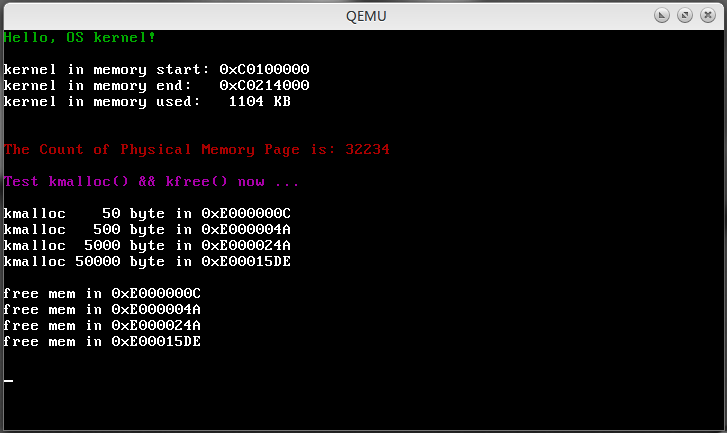
\includegraphics[scale=0.6]{picture/chapt11/HEAP_TEST.png}
      \caption{测试内核堆管理函数}
\end{figure}

\par OK,任务完成!
